\documentclass[11pt,leqno]{article}
\usepackage[polish]{babel}
\usepackage[utf8]{inputenc}
\usepackage{polski}
\usepackage{a4wide}
\usepackage{graphicx}
\usepackage{amsmath,amsthm}
\usepackage{bbm}
\usepackage{bm}
\usepackage{epstopdf}
\usepackage{color}
\usepackage{listings}
\usepackage{fancyhdr}
\usepackage[a4paper,footskip=72pt,headheight=0pt,headsep=0pt]{geometry}

%%%%%%%%%%%%%%%%%%
% Bajery skopiowane z przykładowej pracowni: http://www.ii.uni.wroc.pl/~pwo/An/przykladowe_sprawozdanie.zip
%%%%%%%%%%%%%%%%%%
% Kropka po numerze paragrafu, podparagrafu itp.

\newcommand{\projectName}{NCMA}%\%TempName\% 
\makeatletter
\let\ps@plain\ps@fancy
 \renewcommand{\headrulewidth}{0pt}
\makeatother

\title{\vspace{-3cm} {\bf \projectName \\ {\it \small Nicolas Cage Mega Analyser}}}
\author{Pan Kleszcz \& Chudy}
\date{Wrocław, \today\\
{\small v.1.0.0.3 rc1}}

\pagestyle{fancy}
\fancyhf{}
\fancyfoot[CE,CO]{
\includegraphics[width=\textwidth]{loga}
{\bf Projekt współfinansowany przez Unię Europejską ze środków Europejskiego Funduszu Społecznego w ramach projektu Kapitał Ludzki}\\ \thepage}


\begin{document}
\maketitle
%\thispagestyle{empty}
%\newpage
%\tableofcontents
%\newpage
% 		Ok, najtrudniejsze za nami.		%

\section{Wstęp}	%%%%%%%%%%%%%%%%%%%%%%%%%%%%%%%%%%%%%%%%%%%%%%%%%%%%%%%%%%%%%%%%%%%%
The following file contains the documentation of the project {\bf \projectName}.
The aim is to develop a mindstate recognition system.
It should react to brainwaves that are specific to motoric and telekinepathologic functions.
Apart from research on applications of Mexican cuisine in industry, the system should use information gathered from brainwaves to direct a performance.

\vspace{1cm}

{\it Project endorsed by National Council for Mentalists and Antechamberlains}
\newpage
\section{Technical details}
\subsection{Software}
NCMA is written in Python 2.7 enriched by a bunch of libraries.
TODO libraries
Version control system -- Git.

\subsection{Style sheet}
Indentation: 4 spaces.
Tabulation must not be used.
If the code is wider than split screen allows you to, then the code is bad.
\newpage
\section{Modules}

\begin{center}
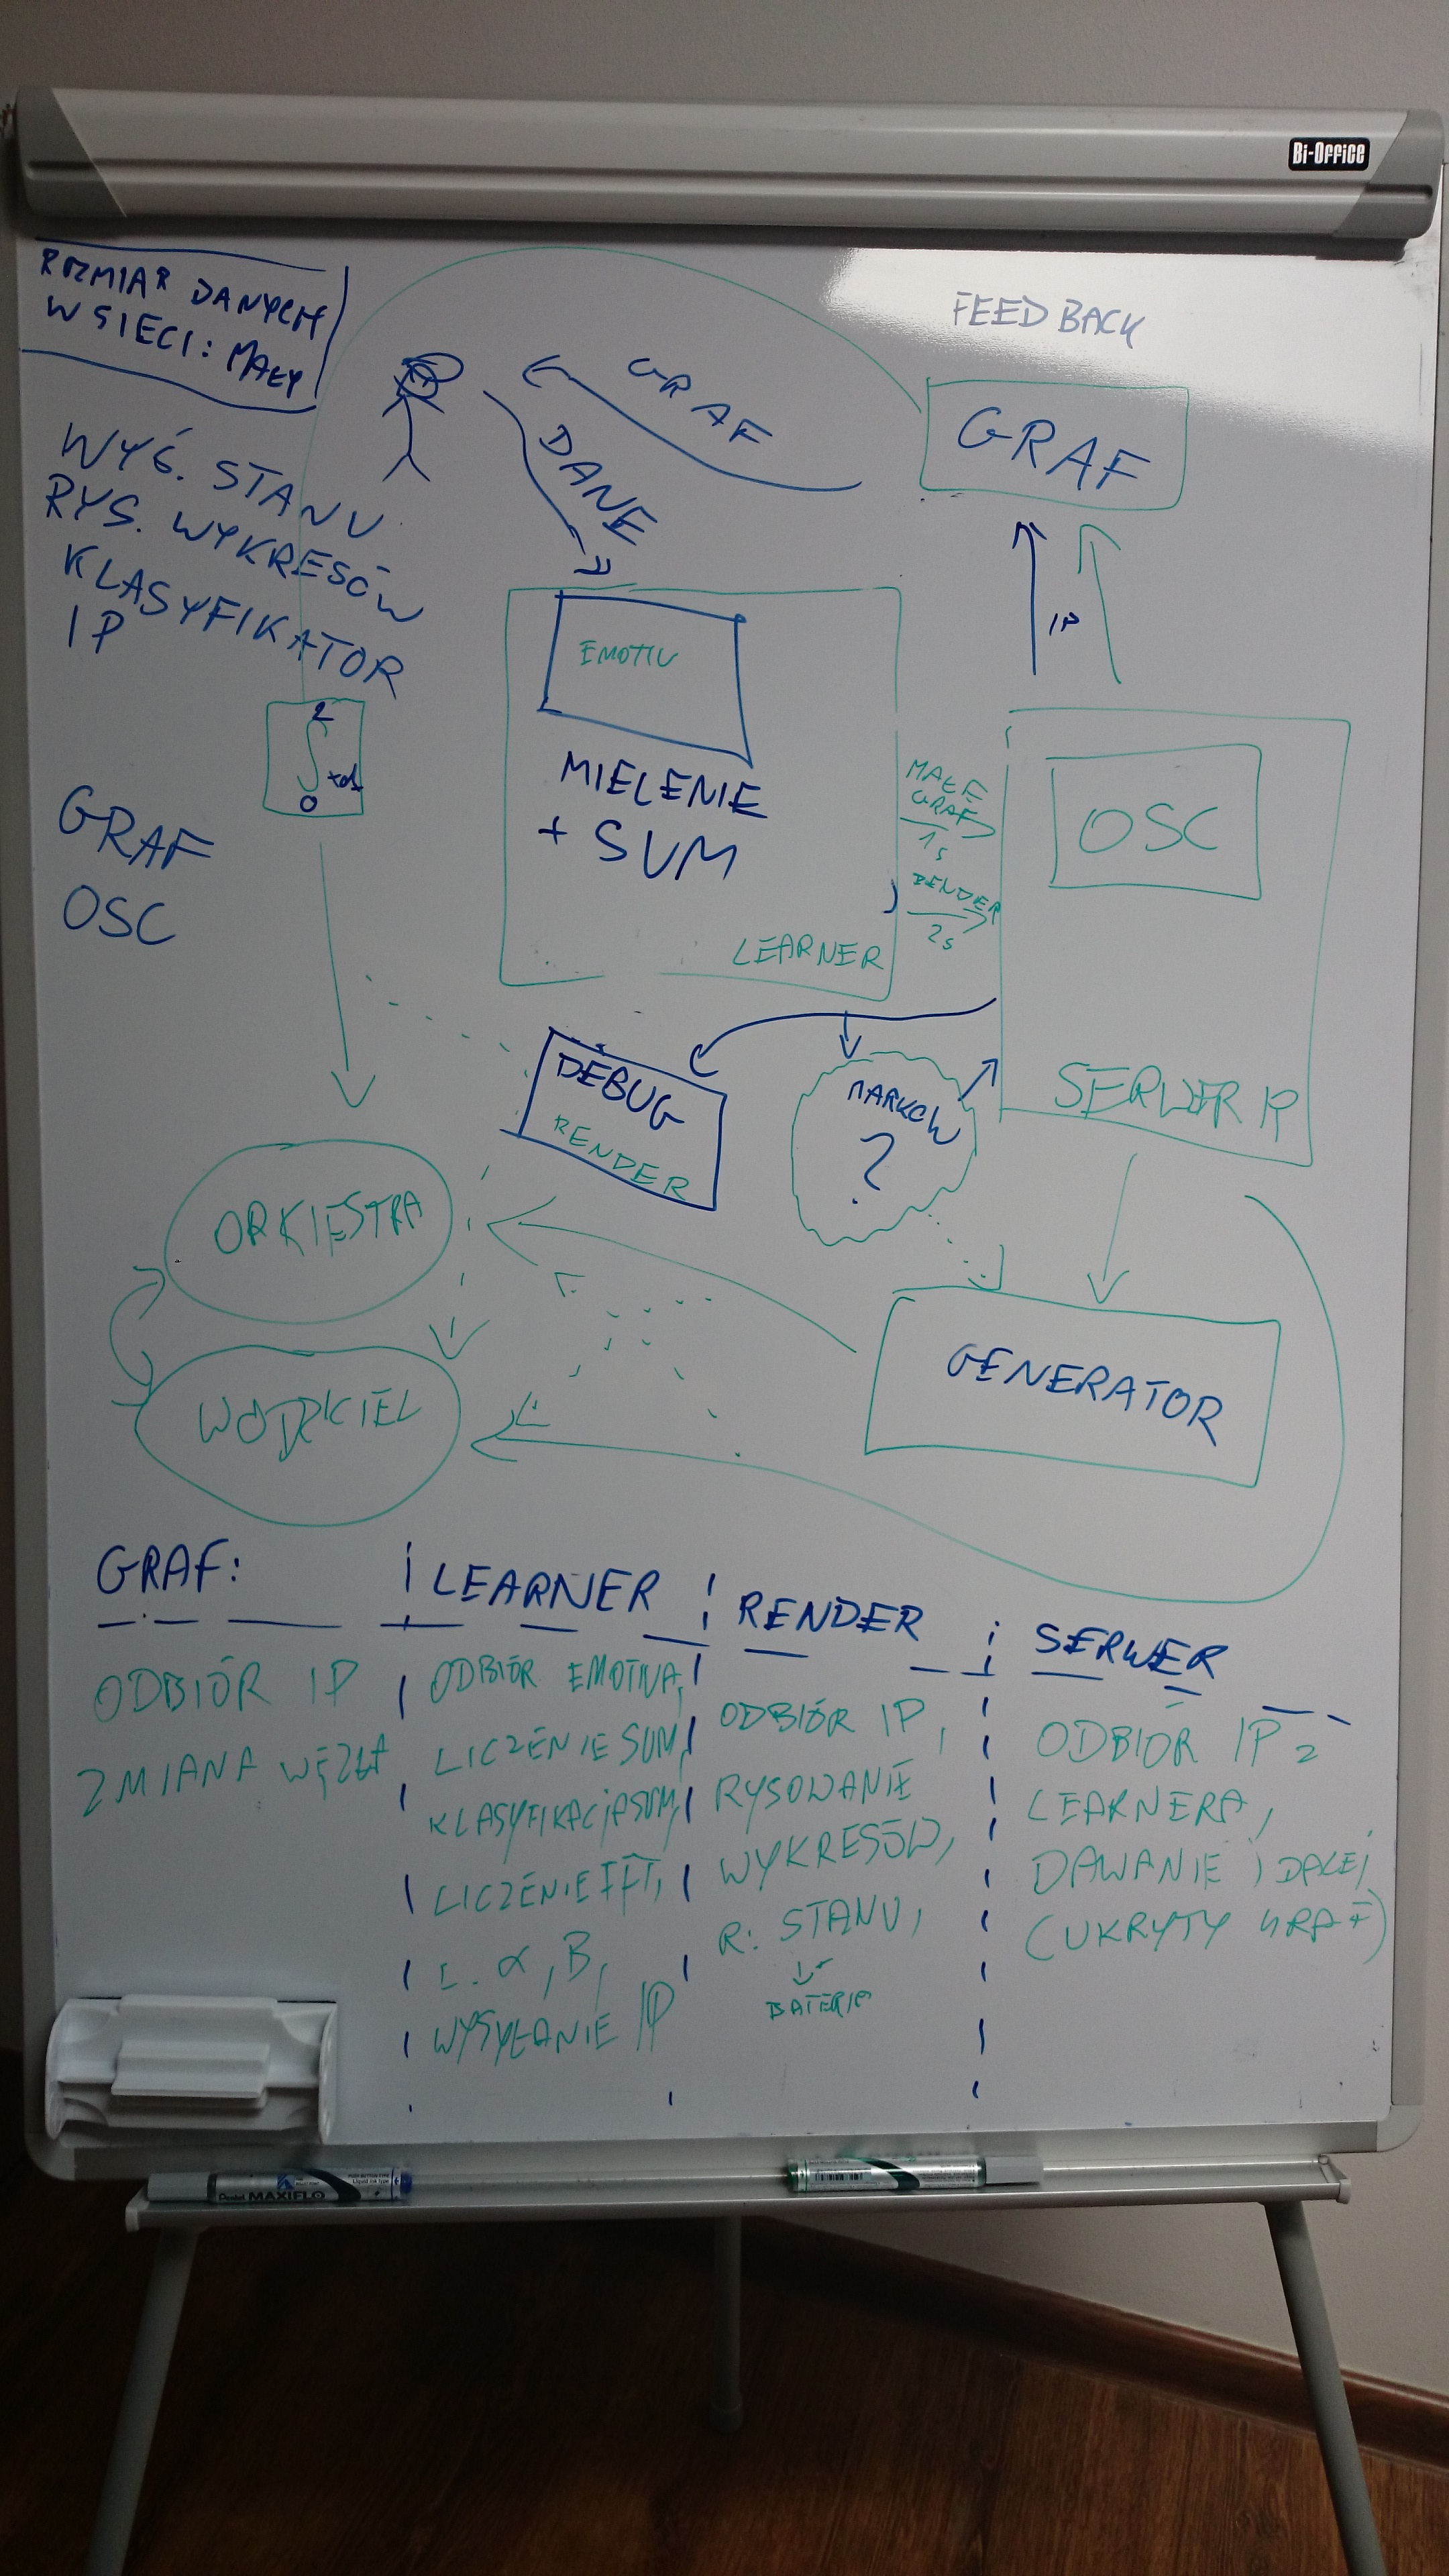
\includegraphics[height=\textheight]{zadania}
\end{center}
\newpage
\subsection{Example}
\begin{lstlisting}[language=Python,frame=single]
for i in range(1,l-1):
    derivs.append((values[i+1] - values[i-1]) / 
        (2 * sampling_period))
\end{lstlisting}   

\end{document}

